\documentclass[12pt]{article}
\usepackage[margin=1in]{geometry}
\usepackage{fourier}
\usepackage{graphicx}
\usepackage[import]{xypic}
\usepackage{tikz}
\usetikzlibrary{braids}
\usetikzlibrary{calc}
\usetikzlibrary{arrows.meta}
\usetikzlibrary{decorations.markings}
\usetikzlibrary{decorations.pathreplacing}
\usepackage[colorlinks=true, linkcolor=blue, citecolor=blue, urlcolor=blue]{hyperref}

\newenvironment{xyoverpic}[3]
{%
\begin{xy}
\xyimport#1{\includegraphics[#2]{#3}}
}{\end{xy}}

\newenvironment{cxyoverpic}[3]
{%
\begin{center}
\centering\leavevmode\large
\begin{xyoverpic}{#1}{#2}{#3}
}{\end{xyoverpic}
\end{center}}

\setlength{\parindent}{0pt}

\begin{document}
\section{Conventions for crossings}\label{sec:cross}

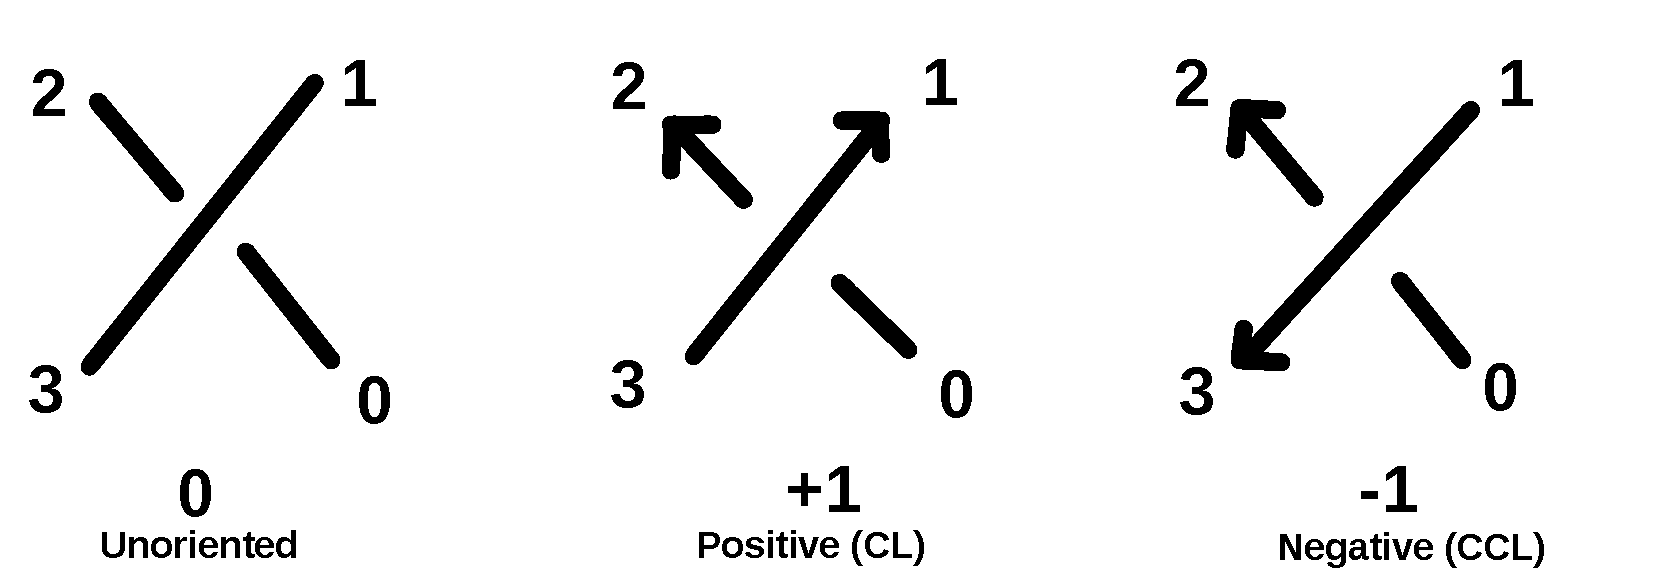
\includegraphics[scale=0.6]{pics/crossings}



\section{Conventions for tangles}

A tangle $T$ is a rectangular piece of a projection with $2n$ incoming
strands, where these strands are numbered as shown.

\begin{cxyoverpic}{(216,144)}{scale=1.0}{pics/tangle}
    ,(107,72)*{T}
    ,(39,14)*++!U{0}
    ,(64,13)*++!U{1}
    ,(84,13)*++!U{2}
    ,(156,13)*++!U{n-2}
    ,(179,13)*++!UL{n-1}
    ,(39,130)*++!DR{n}
    ,(62,131)*++!D{n+1}
    ,(155,132)*++!D{2n - 2}
    ,(178,132)*++!DL{2n - 1}
\end{cxyoverpic}


Conventions for operations and rational tangles follow

 \url{http://homepages.math.uic.edu/~kauffman/VegasAMS.pdf}

 and are shown on the next page.

\pagebreak 

\begin{cxyoverpic}{(432,576)}{scale=1.0}{pics/tangles}
    ,(74,439)*{T + S}
    ,(183,418)*{T \ast S}
    ,(273,484)*{\mbox{\scriptsize cross.}}
    ,(273,500)*{\mbox{\scriptsize mirror}}
    ,(270,445)*{-T}
    ,(354,440)*{\displaystyle\frac{1}{T}}
    ,(81,285)*{T \, \big\vert \, S}
    ,(231,282)*{\mbox{\normalsize Numerator closure}}
    ,(352,282)*{\mbox{\normalsize Denominator closure}}
    ,(20,235)*+!L{\mbox{\textbf{Basic rational tangles}}}
    ,(71,164)*{-2}
    ,(145,164)*{-1}
    ,(209,164)*{0}
    ,(282,164)*{1}
    ,(363,164)*{2}
    ,(69,76)*{\displaystyle -\frac{1}{2}}
    ,(152,76)*{\displaystyle-\frac{1}{1}}
    ,(212,74)*{\infty}
    ,(280,77)*{\displaystyle\frac{1}{1}}
    ,(364,74)*{\displaystyle\frac{1}{2}}
\end{cxyoverpic}


\section{Conventions for braids}

The convention for SnapPy 3.0/Spherogram 2.0 and newer is illustrated
by the braid closure of $\sigma_1^3 \sigma_2^{-2} \sigma_3$
corresponding to \verb+Link(braid_closure=[1, 1, 1, -2, -2, 3])+.
Note that a positive braid has all positive crossings in the sense of
Section~\ref{sec:cross}.

\begin{center}
  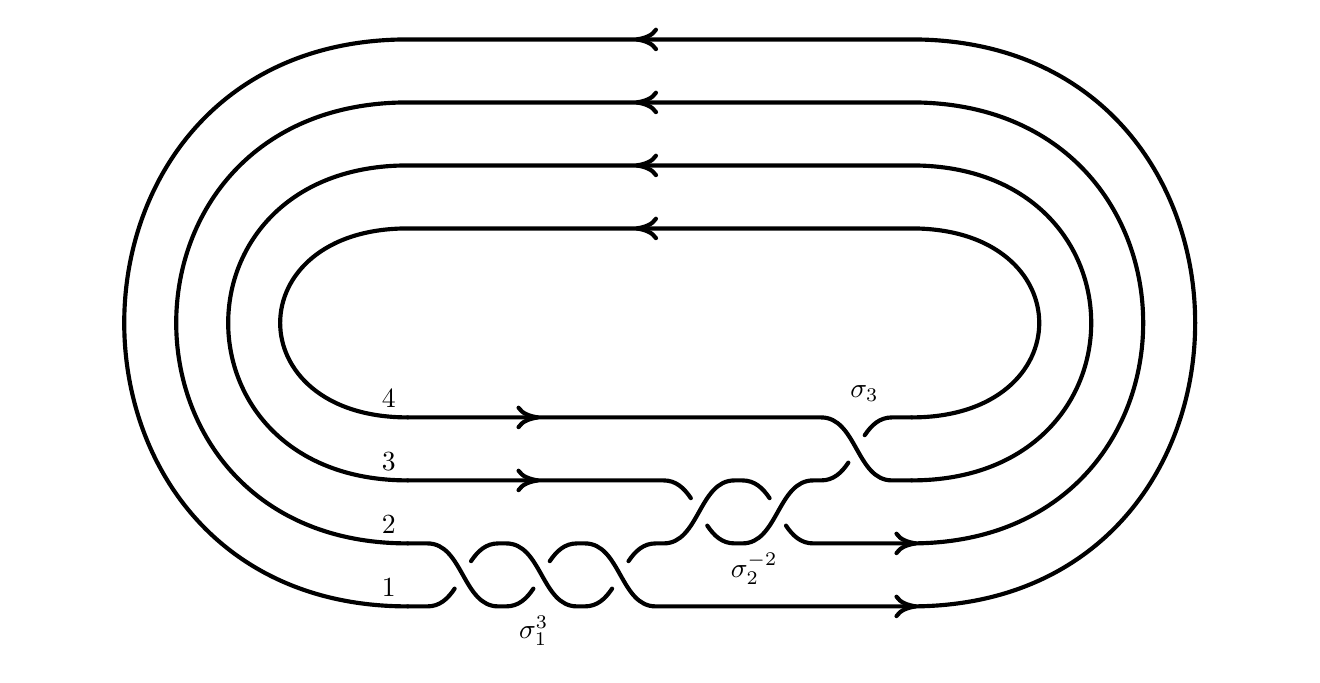
\begin{tikzpicture}[scale=0.8,
    >={Computer Modern Rightarrow[length=1pt 5, width'=0pt 1]}]
  \begin{scope}[line width=1.5pt, line cap=round]
    \foreach \y in {0, 1, 2, 3}{
      \coordinate (a) at (0, \y);
      \coordinate (b) at ($(0, 9) - (a)$);
      \coordinate (c) at ($(8, 9) - (a)$);
      \coordinate (d) at ($(8, 0) + (a)$);
      \coordinate (t) at ($(-6, 0) + 1.1*(\y, 0)$);
      \coordinate (s) at ($(6, 0) +  1.1*(-\y, 0)$);
      \draw (a) .. controls +(t) and +(t) .. (b) --
            (c) .. controls +(s) and +(s) .. (d);
      \draw[<-] ($(c)!0.55!(b)$) -- +(0.1, 0); 
    }
    \draw[->] (2, 3) -- +(0.1, 0); 
    \draw[->] (2, 2) -- +(0.1, 0);
    \draw[->] (8, 1) -- +(0.1, 0); 
    \draw[->] (8, 0) -- +(0.1, 0);
    %\draw (0, 3) .. controls +(-2, 0) and +(-2, 0) .. (0, 6);
    \pic[rotate=90, scale=0.8,
         braid/.cd,
         height=-1.25cm,
         gap=0.15,
         ]
    {braid={s_{2, 1} s_{2, 1} s_{2, 1}
        s_{2, 3} s_{2, 3} s_{4, 3}}};
  \end{scope}
  \foreach \y in {1, 2, 3, 4}{
    \node[above=0.2] at ($(0, \y) + (-0.3, -1)$) {$\y$};
  }
  \node[below] at (2, 0) {$\sigma_1^3$};
  \node[below] at (5.5, 1) {$\sigma_2^{-2}$};
  \node[above] at (7.25, 3.1) {$\sigma_3$};
\end{tikzpicture}
\end{center}



In earlier versions of SnapPy, the sign of the crossings was reversed,
e.g. the same braid would have been:
\begin{center}
  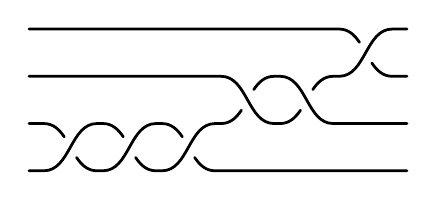
\begin{tikzpicture}
  \begin{scope}[line width=1pt, line cap=round]
    \pic[rotate=90, scale=0.6,
         braid/.cd,
         height=-1.25cm,
         gap=0.15,
         ]
    {braid={s_{1, 2} s_{1, 2} s_{1, 2}
        s_{3, 2} s_{3, 2} s_{3, 4}}};
  \end{scope}
\end{tikzpicture}
\end{center}


\end{document}

